%%%%%%%%%%%%%%%%%%%%%%%%%%%%%%%%%%%%%%%%%
% Thin Sectioned Essay
% LaTeX Template
% Version 1.0 (3/8/13)
%
% This template has been downloaded from:
% http://www.LaTeXTemplates.com
%
% Original Author:
% Nicolas Diaz (nsdiaz@uc.cl) with extensive modifications by:
% Vel (vel@latextemplates.com)
%
% License:
% CC BY-NC-SA 3.0 (http://creativecommons.org/licenses/by-nc-sa/3.0/)
%
%%%%%%%%%%%%%%%%%%%%%%%%%%%%%%%%%%%%%%%%%

%----------------------------------------------------------------------------------------
%	PACKAGES AND OTHER DOCUMENT CONFIGURATIONS
%----------------------------------------------------------------------------------------

\documentclass[a4paper, 11pt]{article} % Font size (can be 10pt, 11pt or 12pt) and paper size (remove a4paper for US letter paper)

\usepackage[protrusion=true,expansion=true]{microtype} % Better typography
\usepackage{graphicx} % Required for including pictures
\usepackage{wrapfig} % Allows in-line images

\usepackage{mathpazo} % Use the Palatino font
\usepackage[T1]{fontenc} % Required for accented characters
%\usepackage[backend=bibtex,style=verbose-trad2]{biblatex}
\usepackage{hyperref}
\usepackage{longtable}
\usepackage{array}
\usepackage{multirow}
\usepackage[utf8]{inputenc}
\usepackage{subcaption}
\usepackage[font=small]{caption}
\usepackage{units}

\linespread{1.05} % Change line spacing here, Palatino benefits from a slight increase by default

\makeatletter
\renewcommand\@biblabel[1]{\textbf{#1.}} % Change the square brackets for each bibliography item from '[1]' to '1.'
\renewcommand{\@listI}{\itemsep=0pt} % Reduce the space between items in the itemize and enumerate environments and the bibliography

\renewcommand{\maketitle}{ % Customize the title - do not edit title and author name here, see the TITLE block below
\begin{flushright} % Right align
{\LARGE\@title} % Increase the font size of the title

\vspace{50pt} % Some vertical space between the title and author name

{\large\@author} % Author name
\\\@date % Date

\vspace{40pt} % Some vertical space between the author block and abstract
\end{flushright}
}

%----------------------------------------------------------------------------------------
%	TITLE
%----------------------------------------------------------------------------------------

\title{\textbf{Specificaties}\\ % Title
Implementaties van koolstofmonoxide sensoren} % Subtitle

\author{\textsc{F. van Beusekom, M. Felida, S. van Bottenburg, J. Grobben, R. Bolding} % Author
\\{\textit{Amsterdam University of Applied Sciences\\ 
HvA\\
Sensor Netwerken: groep 5}}} % Institution

\date{20 September, 2019} % Date

%----------------------------------------------------------------------------------------
\bibliographystyle{IEEEtran}
\begin{document}
\captionsetup[figure]{labelfont={bf},name={Fig},labelsep=period}
\captionsetup{justification=centering}
\hypersetup{hidelinks=true}
\maketitle % Print the title section

%----------------------------------------------------------------------------------------
%	ABSTRACT AND KEYWORDS
%----------------------------------------------------------------------------------------

%\renewcommand{\abstractname}{Summary} % Uncomment to change the name of the abstract to something else


\vspace{10pt} % Some vertical space between the abstract and first section

%----------------------------------------------------------------------------------------
%	ESSAY BODY
%-----------------------------------------------
\newpage
\section{Inleiding}
In dit verslag worden de specificaties besproken van de te ontwikkelen sensor modules voor het project "Sensor Netwerken". Bij dit vak is het de bedoeling dat er low-power sensor modules worden ontwikkeld die de luchtkwaliteit in het HvA gebouw van de faculteit techniek meten en als netwerk informatie uitwisselen met elkaar. Binnen groep 5 is er voor gekozen om koolstofmonoxide te meten (hierna naar gerefereerd als CO), de onderbouwing voor deze keuze staat beschreven in appendix A. Uiteindelijk moet iedereen van deze groep zijn eigen sensor module ontwikkelen. Aangezien het HvA gebouw van de faculteit techniek te vergelijken is met de meeste professionele werkomgeving, wordt er voor dit onderzoek gekeken naar de gebruikelijke CO concentraties in gebouwen en hun uitschieters. Op basis daarvan worden de specificaties opgesteld voor de sensor modules.

\section{Koolstofmonoxide}
Koolstofmonoxide (CO) is een verbinding tussen koolstof en zuurstof. Het is een kleur en geurloos gas. CO komt vrij bij een onvolledige verbranding. Dit kan erg gevaarlijk zijn voor de gezondheid omdat het gas je ongemerkt vergiftigt. Het word dan ook wel eens een "sluipmoordenaar" genoemd. 

\subsection{Ontstaan van CO}
Bij de verbranding van koolstofverbindingen ontstaat er normaal CO2. Als de verbranding onvolledig is, door bijvoorbeeld een tekort aan zuurstof, ontstaat er CO. Een veel voorkomende oorzaak van CO productie zijn niet goed afgestelde of niet goed onderhouden gas kachels en cv-ketels.

\subsection{Effecten op gezondheid}
CO is erg gevaarlijk voor de mens omdat het geur en kleurloos is. Bij inademing van CO word de zuurstofopname verstoord \cite{Effecten Koolmonoxide}. In plaats van zuurstof, bind de CO zich aan de rode bloedcellen. Omdat CO zich sterker hecht aan de rode bloedcellen dan zuurstof, word er minder zuurstof door het lichaam vervoerd. 
\\
De effecten van blootstelling aan CO zijn het gevolg van een zuurstoftekort in het bloed. Hoe meer CO er word opgenomen hoe minder zuurstof er kan worden opgenomen. 

\section{Algemene koolstofmonoxide concentraties}
Het NIVM heeft tussen april 2007 tot en met januari 2008 metingen gedaan in 1028 huishoudens. In 169 van de 1028 huishoudens werden werden er concentraties boven het detectie limiet van 1 \textit{parts per billion} (hierna naar gerefereerd als \textit{ppm}) gevonden. In 8 huishoudens werden er waardes van tussen de 25 en 75 \textit{ppm}, dit waren de meest extreme waardes. in 10 andere huishoudens werden er waardes aangetroffen van tussen de 10 en 25 \textit{ppm} en in de rest van de huishoudens (verreweg de meesten) werden er waardes aangetroffen tussen de 1 en 9 \textit{ppm} \cite{NIVM huurwoningen}. Over een werkdag van 8 uur wordt een tijdgewogen gemiddelde concentratie van 25 \textit{ppm} als grenswaarde aangenomen, over 15 minuten is dit 150 \textit{ppm}. De advies waarden van de Wereldgezondheidsorganisatie (Engels: World Health Organization, WHO) zijn 10 \textit{ppm} als tijdgewogen gemiddelde over 8 uurl en 25 \textit{ppm} over 1 uur \cite{Blootstelling aan CO}.
\subsection{Koolstofmonoxide concentraties in de HvA Leeuwenburg}
Om meer te weten te komen over de huidige manieren van meten van de koolstofmonoxide concentraties in het gebouw van de HvA faculteit techniek, is er contact gezocht het gebouwbeheer. Uit een klein gesprek is gebleken dat er momenteel alleen in de garage CO meters hangen, die wanneer er een bepaalde grenswaarde wordt overschreden (momenteel nog onbekend voor ons welke grenswaarde dat is) alarm slaan waarna vervolgens iedereen de garage moet verlaten.

\section{Luchtkwaliteit meten}
Zoals eerder werd besproken worden de te ontwikkelen sensor modules gebruikt om de luchtkwaliteit te meten. Hierbij wordt dus niet alleen bedoeld om een detector te maken die afgaat na het overschrijden van een bepaalde waarde, maar is het een doel om ook te kunnen meten wanneer je welke concentratie CO in de lucht hebt zitten en hoe ver deze concentratie ligt van de grenswaardes. Binnen groep 5 is afgesproken om de aanname te doen dat de minimale grenswaarde in delen van 1/5e gemeten moet kunnen worden. Aangezien onze sensor modules de hele dag door de CO concentraties in het gebouw moeten meten, gaan we uit van de grenswaarden voor een werk dag (8 uur lang). In dit geval komt de minimale grenswaarde voort uit de Wereldgezondheidsorganisatie (Engels: World Health Organization, WHO) en bedraagt deze 10 \textit{ppm} als tijdgewogen gemiddelde over de hele werkdag. Dit betekend dat wij de CO concentraties willen met een gevoeligheid van 2 \textit{ppm}. Het detectie limiet moet ook 1/5e zijn van de minimale grenswaarde. Dit bedraagt 2 \textit{ppm}.

\section{Specificaties}
\begin{center}
	\begin{tabular}{ | m{5cm} | m{5cm}| } 
		\hline
		\multicolumn{2}{|c|}{Specificaties voor de implementaties van CO sensoren} \\
		\hline
		Meet bereik a: & 0 - 1000 \textit{ppm} \\
		\hline
		detectie limiet:  & 1 \textit{ppm}
		\\ 
		\hline
		detectie resolutie: & 1 \textit{ppm} 
		\\ 
		\hline
		response tijd: & < 1 minuut
		\\ 
		\hline
		Voed spanning: & min: 2,7V max: 3,3V
		\\ 
		\hline
		Maximaal vermogen: & 1 mW
		\\
		\hline
		Output gevoeligheid: & 1mV/\textit{ppm}
		\\
		\hline
	\end{tabular}
\end{center}

\newpage
\appendix
\section{Appendix A: NOx onderzoek}
Stikstofoxides zijn verbindingen tussen stikstof en zuurstof in de vormen $NO$ en $NO_2$. Stikstofdioxide ($NO_2$) komt vrij bij de verbranding van fossielen brandstoffen. In Nederland zijn de grootste uitstoters van $NO_x$ het verkeer en de elektriciteitscentrales.  De uitstoot van $NO_2$ heeft gevolgen voor de natuur en de gezondheid. $NO_2$ word dan ook vaak gebruikt als indicator van de luchtkwaliteit.

\subsection{Effecten van NOx}
Stikstofoxide levert een bijdrage aan de vorming van zure regen. Blootstelling aan $NO_2$ hangt samen met luchtwegklachten zoals verminderende longfunctie, astma-aanvallen en infecties. $NO$ daarin tegen heeft weinig gezondheidseffecten \cite{NO2_Amsterdam}. 


\subsubsection{Normen}
De norm voor het jaargemiddelde $NO_2$ is 	$40\,\nicefrac{\mu g}{m^{3}}$. Deze norm wordt lokaal enkele keren per jaar overschreden. Omdat het verkeer veel $NO_2$ uitstoot, geld een maximaal toegestaan uurgemiddelde van $200\,\nicefrac{\mu g}{m^{3}}$ voor wegen waar meer dan 40.000 motorvoertuigen per etmaal gebruik van maken.

\begin{center}
	\begin{tabular}{ | m{5cm} | m{5cm}| } 
		\hline
		Soort norm & Concentratie \\
		\hline
		Jaargmiddelde & $40\,\nicefrac{\mu g}{m^{3}}$
		\\ 
		\hline
		Uurgemiddelde & $200\,\nicefrac{\mu g}{m^{3}}$* 
		\\ 
		\hline
	\end{tabular}
\end{center}

\begin{footnotesize} 
	* Van toepassing voor wegen waarvan ten minste 40.000 motorvoertuigen per etmaal gebruik maken.
\end{footnotesize}

De gemiddelde concentratie $NO_2$ in de Amsterdamse buitenlucht ligt rond de $25\,\nicefrac{\mu g}{m^{3}}$ (13 ppb). De concentraties binnen liggen meestal een factor 2 lager dan buiten. 

\begin{figure}
	\centering
	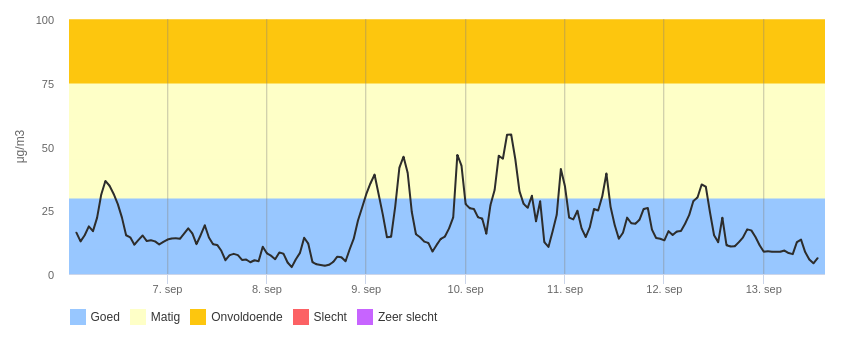
\includegraphics[width=.9\linewidth]{../Old/NO2_doc/amsterdam.png}
	\caption{Meetwaardes $NO_2$ Kantershof Amsterdam zuidoost. 6 tot 11 september 2019 \cite{grafiek}}
	\label{fig:grafiek}
\end{figure}

\newpage
\subsubsection{Sensoren}
Om de voorkomende niveau's te kunnen meten moet de gekozen sensor een meetbereik hebben tussen de 0 en de 40 ppb, met een resolutie van 1 ppb.\\
De NO2-B43F $NO_2$ sensor is een chemoresistive sensor van Alphasense en lijkt de beste optie maar is niet geschikt.\\
Deze sensor een meetbereik van 0 tot 20 ppm met een meetonzekerheid van 15 ppb. Deze sensor is niet gevoelig genoeg om de lage concentraties met een resolutie van 1 ppb uit de lucht goed te kunnen meten.\\ 
Sensoren die $NO_2$ meten hebben een kruisgevoeligheid voor andere gassen zoals $O_3$ en zijn erg gevoelig voor veranderingen in temperatuur en luchtvochtigheid. \\
De sensor moet energie zuinig zijn waardoor chemoresistive sensoren niet geschikt zijn omdat deze een continu verbruik is in de ordegrootte van 50 mW \cite{B4DF}. 

\subsubsection{Conclusie}
Er is geen sensor op de markt beschikbaar om de concentraties $NO_2$ die we verwachten te meten. De beschikbare sensoren zijn niet gevoelig genoeg en verbruiken te veel energie. Daarom is er voor gekozen om af te stappen van het meten van $NO_2$ als indicator van de luchtkwaliteit binnen de HvA gebouwen. Als alternatief is gekozen voor het meten van $CO$ concentraties in de lucht. $CO$ is een giftig gas en kan vrijkomen bij onvolledige verbrandingen en is daarom belangrijk om dit gas tijdig te registreren.
%----------------------------------------------------------------------------------------
\newpage
\begin{thebibliography}{9}
	\bibitem{Effecten Koolmonoxide}
	Mariët Ticheler, 
	2008 [Bekeken in september 2019],
	[Rapport],
	"Koolmonoxide",
	Beschikbaar: \url{https://www.leefmilieu.nl/sites/www3.leefmilieu.nl/files/imported/pdf_s/MGM_2008-02_koolmonoxide.pdf}
	
	\bibitem{NIVM huurwoningen}
	M. van Bruggen, J.T.M. Gram, E.L. Boels, L. Ruhaak, M. Mooij,
	NIVM,
	2009 [Bekeken in september 2019],
	[Rapport],
	"Koolmonoxide in huurwoningen in de Randstad",
	Beschikbaar: \url{https://www.rivm.nl/bibliotheek/rapporten/609300009.pdf}
	
	\bibitem{Blootstelling aan CO}
	M. Mooij,
	NIVM,
	2008 [Bekeken in september 2019],
	[Rapport],
	"Chronische blootstelling aan koolmonoxide, tabel 2.2",
	Beschikbaar: \url{https://www.rivm.nl/bibliotheek/rapporten/609300005.pdf}
	
	\bibitem{NO2_Amsterdam}
	RIVM, J.p. Wesseling, S. van der Zee, P.L. Nguyen,
	2008 [Bekeken in september 2019],
	[Rapport],
	"Gemeten en berekende NO2-concentraties in Amsterdam in 2008",
	Beschikbaar: \url{https://www.rivm.nl/bibliotheek/rapporten/680705015.pdf}
	
	\bibitem{grafiek}
	Rijksinstituut voor Volksgezondheid
	2019[Bekeken in september 2019],
	[Online],
	"Meetgegevens NO2",
	Beschikbaar: \url{https://www.luchtmeetnet.nl}
	
	\bibitem{B4DF}
	Alphasense
	2018[Bekeken in september 2019],
	[Datasheet],
	"Datasheet",
	Beschikbaar: \url{http://www.alphasense.com/WEB1213/wp-content/uploads/2018/12/NO2B43F.pdf}
\end{thebibliography}

\end{document}
